\documentclass[aspectratio=169]{beamer}

\usepackage[ngerman]{babel}
\usepackage[utf8]{inputenc}
\usepackage{tikz}
\usepackage{graphicx}
\usepackage{array}
\usepackage{booktabs}
\usepackage{amsmath}

\usetheme{aig}

\title{Stimmungsanalyse mit Twitter}
\author[Team Twitter Sentiment]{Anne Huber, Andreas Franke, Felix Lindner, Burak Özkan, Milomir Soknic}
\institute{Projektpraktikum Web Science,\\Artificial Intelligence Group,\\Universität Hagen, Deutschland}
\date{18. März 2025}

\begin{document}

\begin{frame}
	\titlepage
\end{frame}

\begin{frame}{Motivation}
	\begin{columns}
		\column{0.5\textwidth}
		\centering
		
\includegraphics[scale=0.2]{Tweets.png}

		\column{0.5\textwidth}
		\begin{itemize}
			\item Twitter als Echtzeit-Plattform für Meinungen und Trends
			\item Große Datenmengen für maschinelles Lernen nutzbar
			\item Herausforderungen: Ironie, Sarkasmus, Emojis, Abkürzungen
			\item Einsatz in Politik, Marketing und Krisenmanagement
		\end{itemize}
	\end{columns}
\end{frame}

\begin{frame}{Zielsetzung}
	\Large
	\begin{itemize}
		\item Wie effektiv sind verschiedene maschinelle Lernverfahren bei der Stimmungsanalyse von Tweets?
	\end{itemize}
\end{frame}


%=========================================================================================================================
\section{Daten}


\subsection{Datenauswahl}

\begin{frame}{Daten - Datenauswahl}
	\begin{itemize}
		\item Prüfung diverser Datensätze
		\item Entscheidung für \glqq Sentiment140\grqq
		\item Besonderheiten:
		      \begin{itemize}
			      \item Artikel: \glqq Twitter Sentiment Classification using Distant Supervision\grqq
			      \item Bessere Datenqualität
			      \item Ausbalancierte Klassen
			      \item Emoticons als Sentiment-Indikatoren
		      \end{itemize}

		      \vspace{0.5cm}
		      \textbf{Beispieltweet:}
		      \vspace{0.2cm}

		      \begin{figure}
			      \centering
			      \begin{columns}[T]
				      \begin{column}{0.45\textwidth}
					      \centering
					      \textbf{Original Tweet}\\
					      \textit{Just got my dream job! So excited! \yellowhighlight{:)}}
					      \vspace{0.5cm}
				      \end{column}

				      \begin{column}{0.1\textwidth}
					      \centering
					      \LARGE $\Rightarrow$
				      \end{column}

				      \begin{column}{0.45\textwidth}
					      \centering
					      \textbf{Datensatz}\\
					      \textit{Just got my dream job! So excited!} \\
					      \vspace{0.2cm}
					      \textbf{Stimmung: \yellowhighlight{Positiv}}
					      \vspace{0.5cm}
				      \end{column}
			      \end{columns}
		      \end{figure}

	\end{itemize}
\end{frame}


\subsection{Testdatensatz}

\begin{frame}{Daten - Testdatensatz}
	\textbf{Eigenschaften:}
	\begin{itemize}
		\item Enthält \textbf{359} manuell gesammelte Tweets
		\item \textbf{177} negative und \textbf{182} positive Tweets
		\item Keine automatische Annotation durch Emoticons
		\item Dient zur unabhängigen Evaluierung von Modellen
		\item Testdatensatz enthält zusätzlich \textit{Query-Terms}
	\end{itemize}

	\vspace{0.5cm}
	\textbf{Beispieltweet:}

	\begin{center}
		\glqq \textit{no. it is too big. I'm quite happy with the \yellowhighlight{Kindle2}\grqq}
		\vspace{0.25cm}
		\begin{columns}
			\begin{column}{0.45\textwidth}
				\textbf{Ohne Query Term: \darkhighlight{Negativ}}
			\end{column}
			\begin{column}{0.45\textwidth}
				\textbf{Mit Query Term: \darkhighlight{Positiv}}
			\end{column}
		\end{columns}
	\end{center}
\end{frame}


%=========================================================================================================================
\section{Klassische Methoden}

\begin{frame}{Klassische Methoden - Überblick}
	\fontsize{10pt}{12pt}\selectfont
	\vspace{0.3cm}

	\begin{columns}[t]
		\column{0.45\textwidth}
		\textbf{Klassische Methoden}
		\vspace{0.3cm}
		\begin{itemize}
			\item \textbf{Logistische Regression}
			\item \textbf{\textit{Support Vector Machine (SVM)}}
			\item \textbf{Naiver Bayes}
			\item \textcolor{gray}{Entscheidungsbäume}
			\item \textcolor{gray}{Entscheidungswälder}
			\item \textcolor{gray}{K-nächste Nachbarn}
		\end{itemize}
		\vspace{0.5cm}
		\textbf{Metrik:} Genauigkeit
		\vspace{-0.5cm}
		\column{0.55\textwidth}
		\textbf{Parameter}
		\vspace{0.3cm}
		\begin{itemize}
			\item Vektorisierungsmethode
			\item Normalisierungsstrategie
			\item Strategie zur Entfernung von Stoppwörtern
			\item N-Gramm-Bereich
			\item Maximale Anzahl an Merkmalen
		\end{itemize}
	\end{columns}
\end{frame}

\begin{frame}{Klassische Methoden - Datenvorverarbeitung}
	\fontsize{10pt}{12pt}\selectfont
	\vspace{0.3cm}

	\begin{table}[]
		\centering
		\renewcommand{\arraystretch}{1.2}
		\begin{tabular}{l|p{7.5cm}}
			\hline
			                                & \textbf{Beispiel}                                                                                   \\
			\hline
			\textbf{Original-Tweet}         & \textit{\glqq @user I love this movie! http://example.com\grqq{}}                                   \\
			\hline
			\textbf{Bereinigung}            & \textit{\glqq I love this movie\grqq}                                                               \\
			\hline
			\textbf{Tokenisierung}          & \textit{[\glqq I\grqq, \glqq love\grqq, \glqq this\grqq, \glqq movie\grqq]}                         \\
			\hline
			\textbf{Transformation}         & Lemmatization: \textit{[\glqq I\grqq, \glqq love\grqq, \glqq this\grqq, \glqq movie\grqq]} \newline
			Stemming: \textit{[\glqq I\grqq, \glqq lov\grqq, \glqq thi\grqq, \glqq movi\grqq]}                                                    \\
			\hline
			\textbf{Stoppwörter Behandlung} & Ohne Stoppwörter: \textit{[\glqq love\grqq, \glqq movie\grq']}                                      \\
			\hline
			\textbf{Merkmalsextraktion}     & TF-IDF Beispiel: \newline
			\textit{(love: 0.75, movie: 0.85)}                                                                                                    \\
			\hline
		\end{tabular}
	\end{table}

\end{frame}

\begin{frame}{Klassische Methode - Beste Genauigkeit pro Modell}
	\centering
	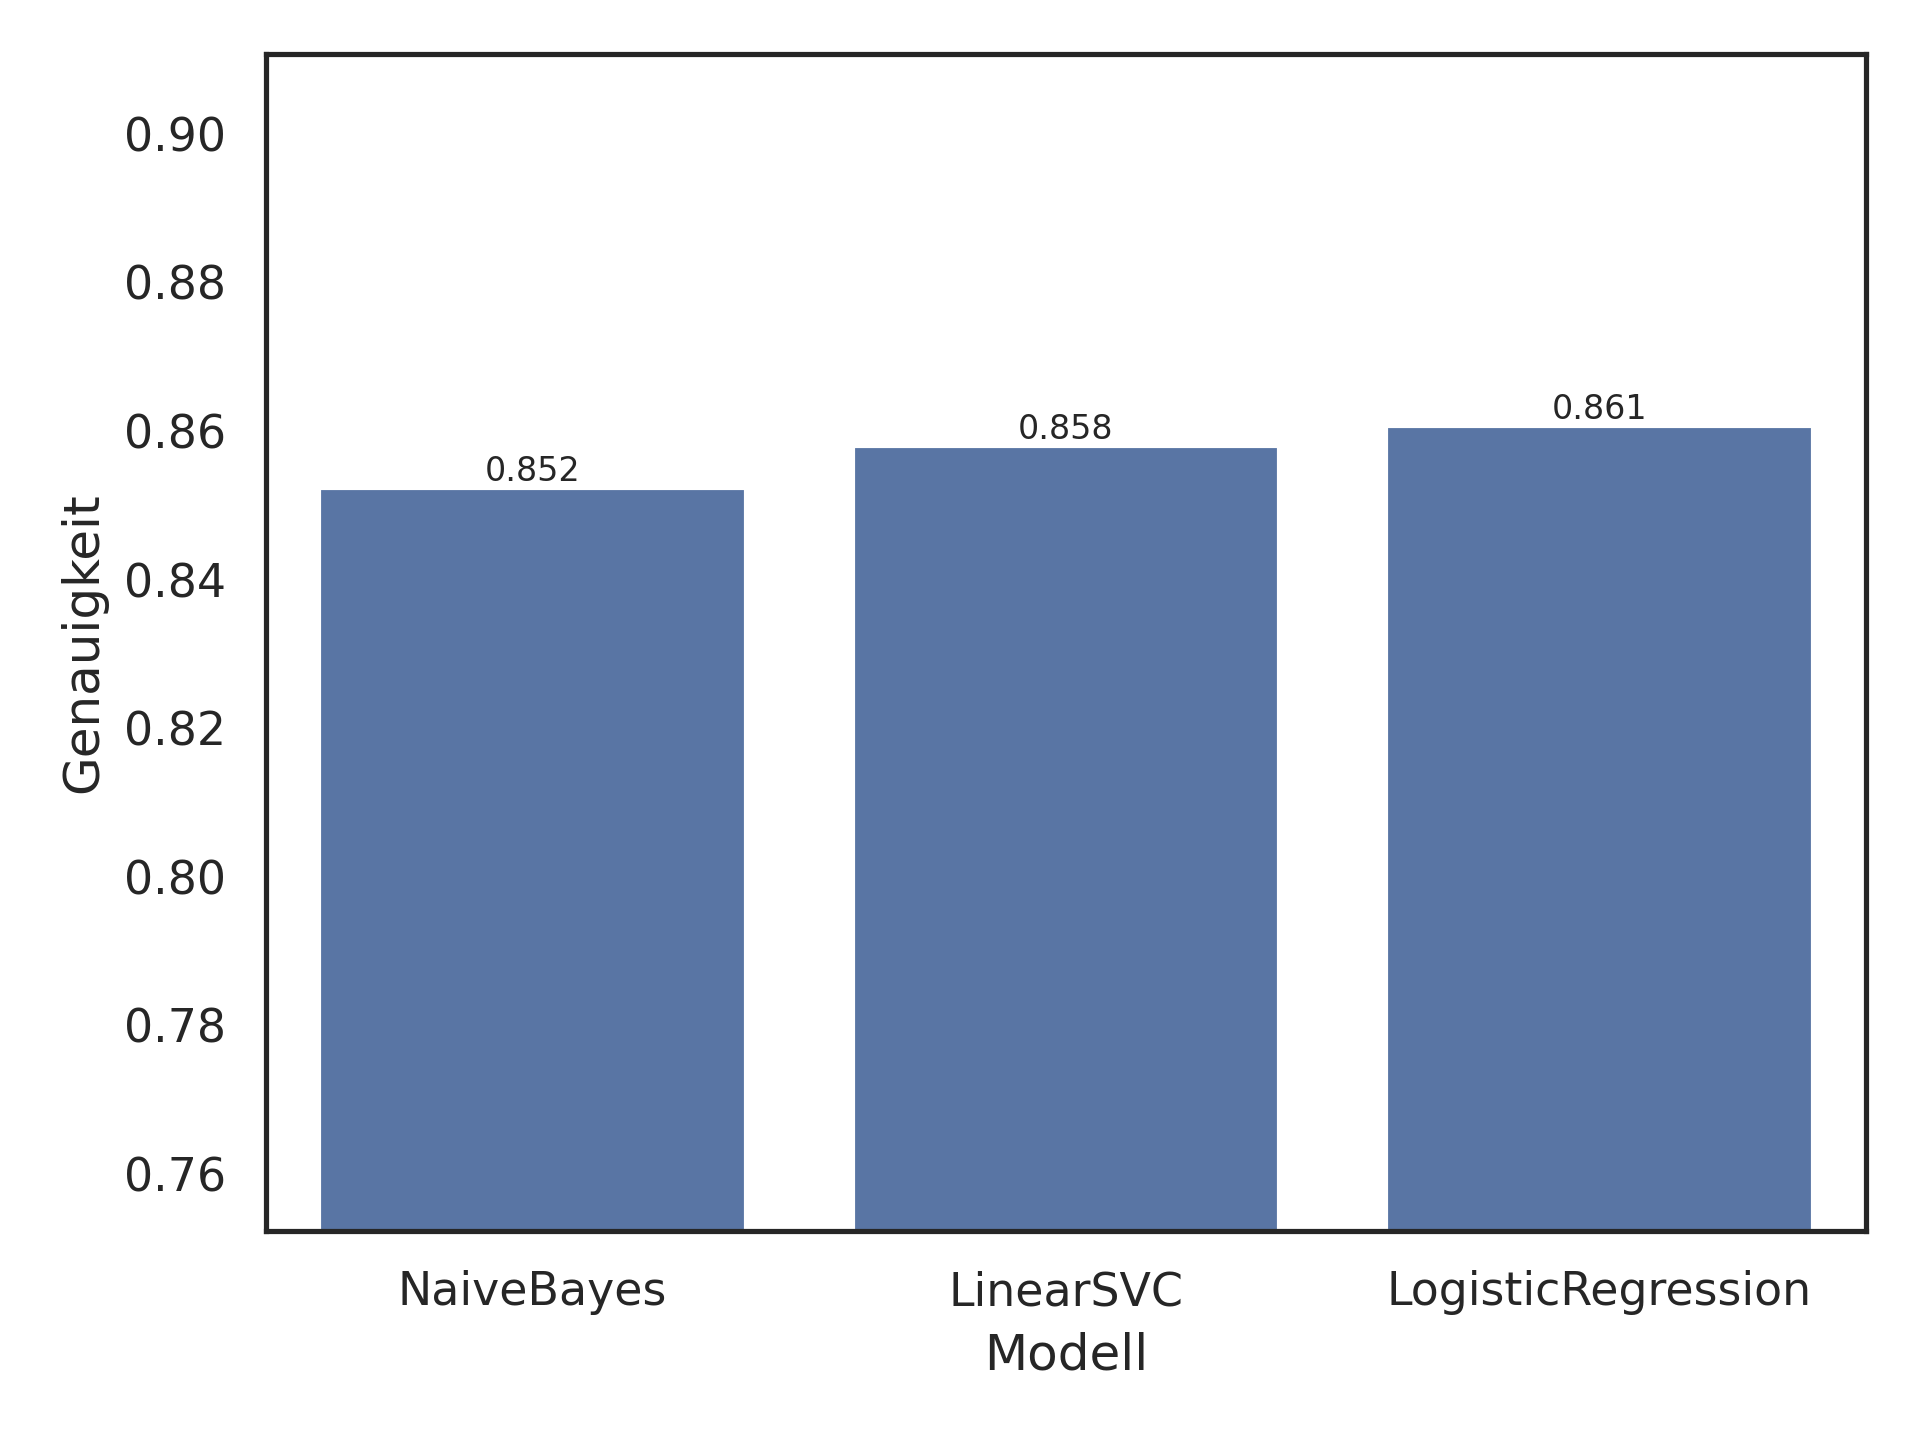
\includegraphics[scale=0.65]{../datasets/sentiment140/results/plots/klassische-ml-beste-genauigkeit-pro-modell-truncated-y-axis.png}
\end{frame}


%=========================================================================================================================
\section{Deep Learning}


\subsection{BERT-Modelle}

\begin{frame}{Deep Learning - BERT-Modelle (1/2)}
	\begin{itemize}
		\item 2018 von Google entwickelt
		\item \textit{Bidirectional encoder representations from transformers} (BERT)
		\item Mit großem textuellen Korpus vortrainiert
		\item 110 Mio. Parameter
		\item Etabliert in der natürlichen Sprachverarbeitung (NLP)
	\end{itemize}
\end{frame}

\begin{frame}{Deep Learning - BERT-Modelle (2/2)}
	\begin{columns}[T]
		\column{0.5\textwidth}
		\begin{block}{DistilBERT-base-uncased}
			\begin{itemize}
				\item Destilliertes BERT-Modell
				\item \textbf{Eigenschaften}:
				      \begin{itemize}
					      \item Modelldestillation des bert-base-uncased Modells
					      \item 40\% kleiner
					      \item 60\% schnellere Inferenz
					      \item 97\% der Fähigkeiten bleiben erhalten
				      \end{itemize}
			\end{itemize}
			\vspace{0.04cm}
		\end{block}
		\column{0.5\textwidth}
		\begin{block}{Twitter-RoBERTa-base-sentiment}
			\begin{itemize}
				\item Auf Twitter-Daten trainiertes RoBERTa-Modell
				\item \textbf{Eigenschaften}:
				      \begin{itemize}
					      \item Mit 58 Mio. englischsprachigen Tweets weitertrainiert
					      \item \textit{Finetuning} mit einem Stimmungsanalyse-Datensatz
				      \end{itemize}
			\end{itemize}
			\vfill
		\end{block}
	\end{columns}
\end{frame}


\subsection{\textit{Finetuning} BERT-Modelle}

\begin{frame}{Deep Learning - \textit{Finetuning} BERT-Modelle}
	\begin{itemize}
		\item \textbf{Methode}
		      \begin{itemize}
			      \item \textit{Finetuning} der Modelle mit Sentiment140
			      \item Huggingface \textit{transformers} Bibliothek
		      \end{itemize}
		\item \textbf{Untersuchte Parameter}
		      \begin{itemize}
			      \item Initiale Lernrate
			      \item Größe des Trainingsdatensatzes
		      \end{itemize}
		\item \textbf{Evaluationsmetrik}
		      \begin{itemize}
			      \item Genauigkeit
		      \end{itemize}
	\end{itemize}
\end{frame}

\begin{frame}{Deep Learning - Ergebnisse BERT-Modelle}
	\centering
	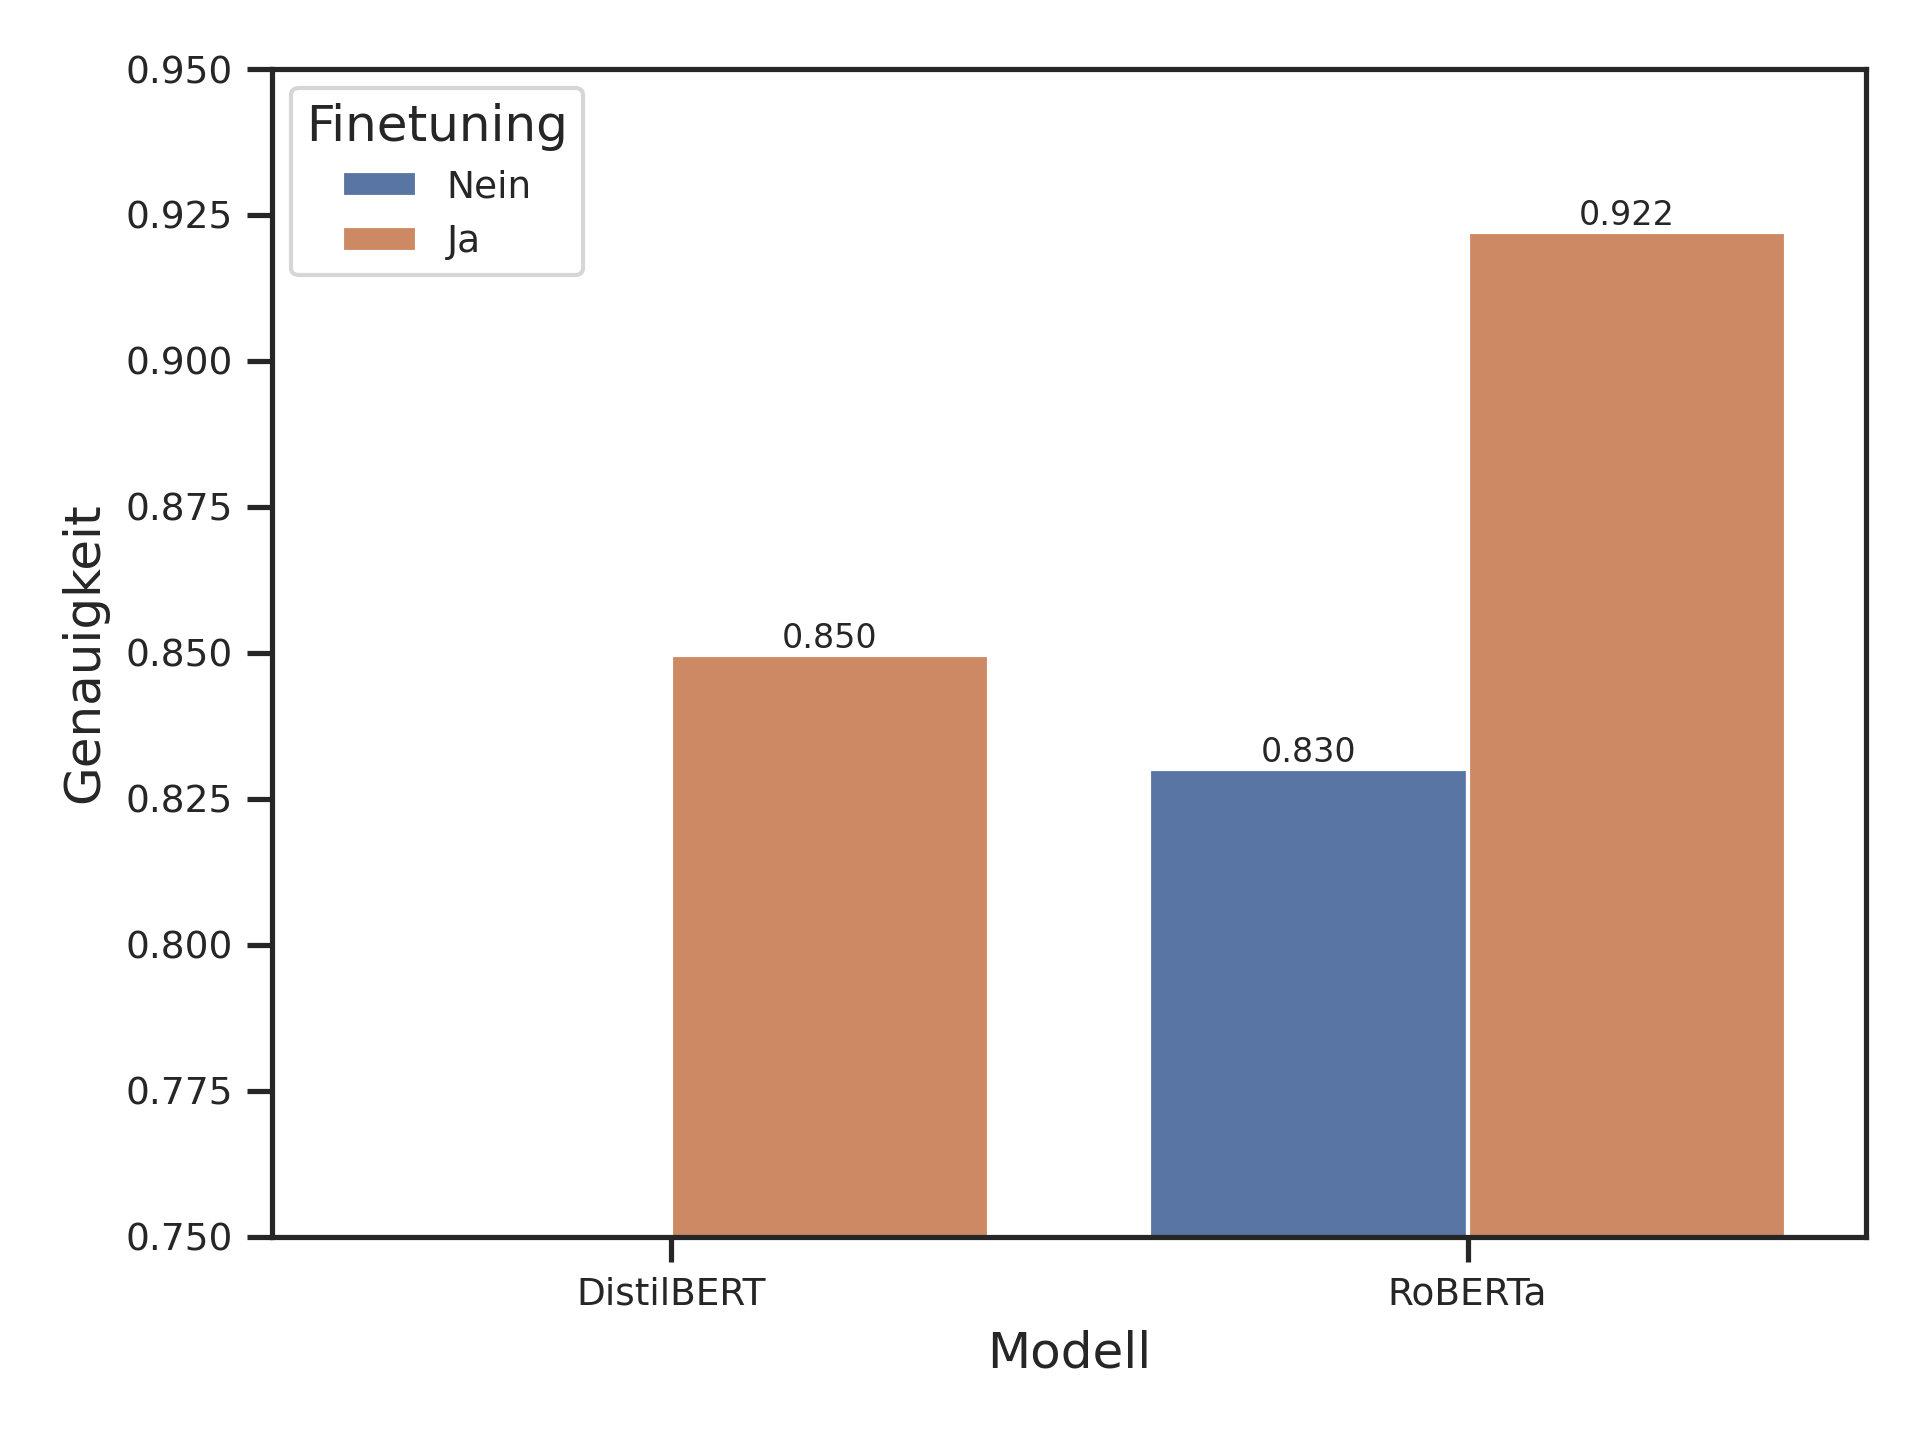
\includegraphics[scale=0.65]{../datasets/sentiment140/results/plots/bert-based-genauigkeit-bert-basierte-modelle-default-vs.-finetuning-truncated-y-axis.png}
\end{frame}


\subsection{DeepSeek}

\begin{frame}{Deep Learning - DeepSeek-R1 Modell}
	\begin{itemize}
		\item \textbf{Reasoning-Modell}
		\item Basiert auf Transformer Architektur
		\item Trainiert mit Hilfe von \textit{Reinforcement Learning}
		\item 671 Mrd. Parameter
		\item Destillierte Modelle verfügbar
	\end{itemize}
	\vspace{0.4cm}

	\begin{itemize}
		\item \textbf{\textit{Finetuning} Ansatz}
		      \begin{itemize}
			      \item \textit{DeepSeek-R1-Distill-Qwen-1.5B}
			      \item Aufgrund von Hardwareanforderungen verworfen
		      \end{itemize}
	\end{itemize}
\end{frame}

\begin{frame}{Deep Learning - DeepSeek-R1 Zero-Shot Ansatz}
	\textbf{Zero-Shot-Ansatz:}

	\vspace{0.35cm}

	\begin{itemize}
		\item Prompt enthält keine Beispiele
		\item Verwendete Modelle
		      \begin{itemize}
			      \item DeepSeek-1.5B
			      \item DeepSeek-8B
			      \item DeepSeek-32B
			      \item DeepSeek-70B
		      \end{itemize}
		\item Inferenz mit und ohne Query-Terms
	\end{itemize}
	\vspace{0.2cm}
	\centering
	\textbf{Prompt:} Tweet sentiment? Sentiment Topic: \{Query-Term\} \\
	Answer with positive or negative. Provide reasoning in JSON.\\
	Tweet: \glqq\{tweet\}\grqq
\end{frame}

\begin{frame}{Deep Learning - DeepSeek-R1 Prompt Beispiel}
	\begin{center}
		\textbf{Tweet:} \glqq \textit{no. it is too big. I'm quite happy with the \yellowhighlight{Kindle2}\grqq}
		\vspace{0.45cm}
		\begin{columns}
			\begin{column}{0.45\textwidth}
				\textbf{Reasoning ohne Query Term} \\
				\vspace{0.4cm}
				\glqq \textit{The tweet expresses dissatisfaction with something being 'too big,' indicating a \darkhighlight{negative sentiment}.\grqq}
			\end{column}
			\begin{column}{0.45\textwidth}
				\textbf{Reasoning mit Query Term:} \\
				\vspace{0.4cm}
				\glqq \textit{The tweet mentions being 'quite happy' with the Kindle2, which indicates a \darkhighlight{positive sentiment}.\grqq}
			\end{column}
		\end{columns}
	\end{center}

\end{frame}

\begin{frame}{Deep Learning - DeepSeek-R1 Ergebnisse}
	\centering
	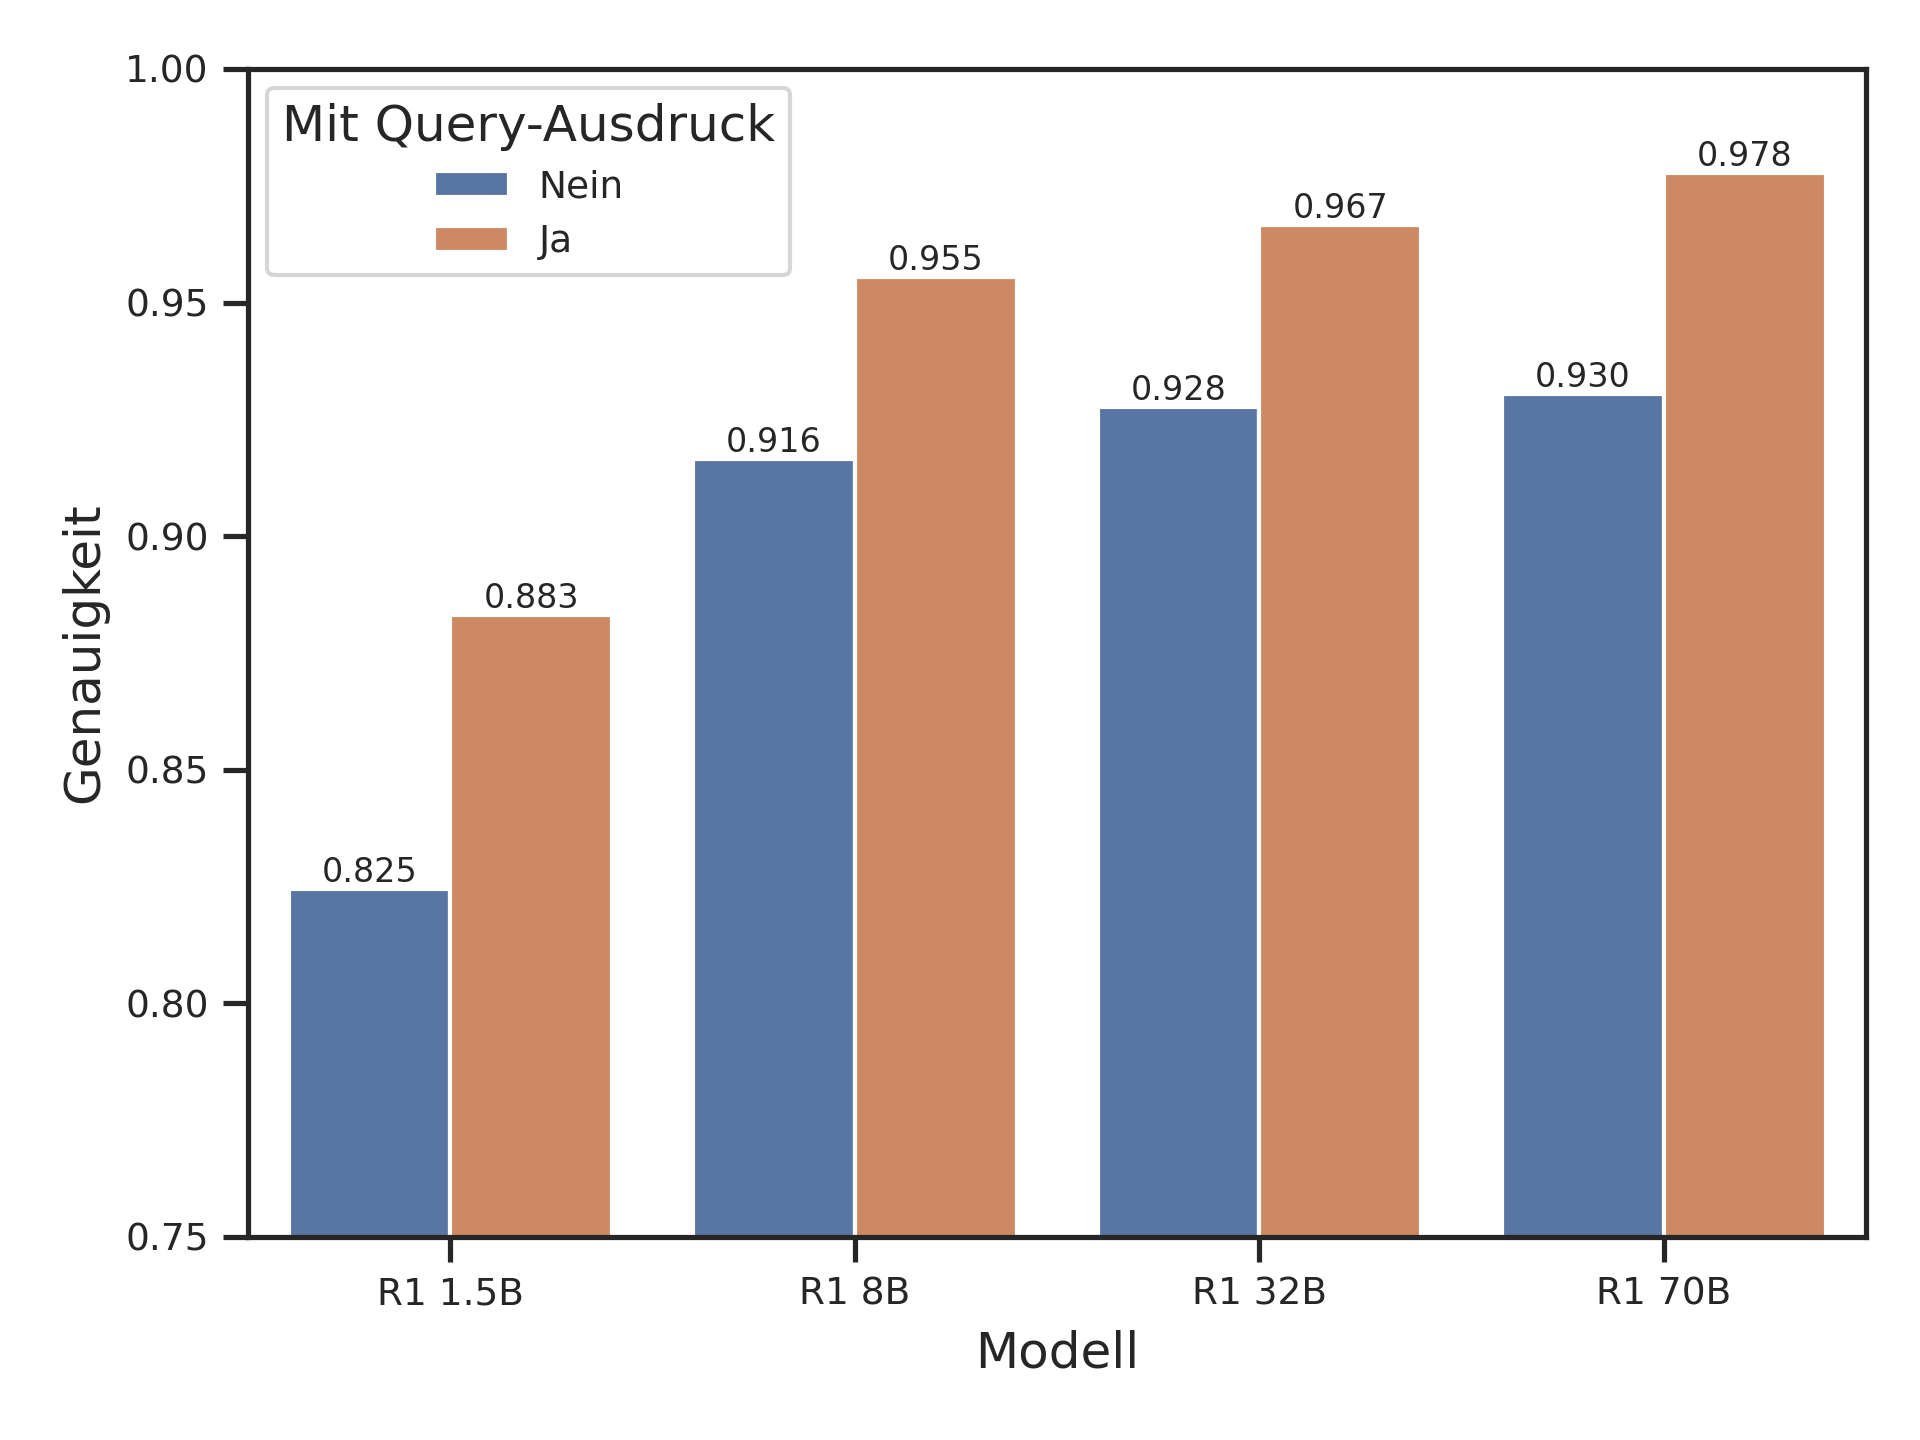
\includegraphics[scale=0.65]{../datasets/sentiment140/results/plots/deepseek-genauigkeit-deepseek-modelle-einfluss-query-ausdruck-truncated-y-axis.png}
\end{frame}


%=========================================================================================================================
\section{Zusammenfassung}

\begin{frame}{Zusammenfassung - Überblick Ergebnisse alle Modelle}
	\centering
	\includegraphics[scale=0.65]{../datasets/sentiment140/results/plots/alle-übersicht-genauigkeit-alle-modelle-truncated-y-axis.png}
\end{frame}

\begin{frame}{Zusammenfassung - Erkenntnisse und Ausblick}
	\normalsize
	\begin{itemize}
		\item \textbf{Erkenntnisse:}
		      \begin{itemize}
			      \item LLMs führen zu höheren Genauigkeiten als klassische Verfahren
			      \item \textit{Finetuning} erhöht Genauigkeit der LLMs
			      \item Query-Terms erhöhen die Genauigkeit für LLMs erheblich
			      \item LLMs haben viel größere Hardwareanforderungen und längere Inferenzzeiten
		      \end{itemize}
		      \vspace{0.4cm}
		\item \textbf{Ausblick:}
		      \begin{itemize}
			      \item \textit{Noisy-Label}
			      \item \textit{Aspect-Based-Sentiment-Analysis} (ABSA)
			      \item Große \textit{Deep Learning} Modelle
		      \end{itemize}
	\end{itemize}

	\vspace{0.5cm}
	\centering
	\pause
	{\large \textbf{Vielen Dank für Ihre Aufmerksamkeit!}} \\[0.1cm]
	\textit{Fragen?}
\end{frame}

\end{document}
